\chapter{Diseño e implementación} % Main chapter title

\label{Chapter3} % Change X to a consecutive number; for referencing this chapter elsewhere, use \ref{ChapterX}

En este capítulo se describen las etapas de diseño y el ajuste del sistema orientado a la clasificación de tareas de imaginación motriz. En las siguientes secciones se detallan la arquitectura del sistema, el tratamiento de los datos de origen, el desarrollo y entrenamiento de los modelos de aprendizaje profundo, así como el protocolo de evaluación y el despliegue final en la infraestructura de la nube.

%----------------------------------------------------------------------------------------
%	SECTION 1
%----------------------------------------------------------------------------------------
\section{Arquitectura del sistema}

En esta sección se describe la arquitectura general del sistema que se utilizó para la predicción de tareas de imaginación motriz a partir de EEG.

El sistema se estructuró como un flujo secuencial compuesto por etapas de preparación de datos, preprocesamiento, extracción de características, inferencia mediante modelos de aprendizaje profundo y despliegue en infraestructura cloud. Este enfoque permitió integrar el procesamiento de señales EEG con servicios distribuidos, facilitando la escalabilidad y la eficiencia en la ejecución de los modelos.

La fuente de datos correspondió al conjunto de datos Dreyer2023A \cite{dreyer2023large}. Este contiene registros de señales EEG asociados a tareas de imaginación motriz. Dicho conjunto fue utilizado como base para el entrenamiento y evaluación de los modelos, sin realizar procesos de adquisición directa de señales.

Luego, se implementó una etapa de preprocesamiento orientada a mejorar la relación entre la señal y el ruido. En esta fase se aplicaron técnicas de filtrado y segmentación, con el fin de aislar ventanas relevantes para el análisis. Este procedimiento permitió reducir la variabilidad inherente a las señales EEG y facilitar el aprendizaje de patrones discriminativos.

La extracción de características se abordó mediante arquitecturas de redes neuronales, que permitieron modelar dependencias espaciales y temporales presentes en las señales. Se consideraron enfoques híbridos capaces de capturar correlaciones entre canales y dinámicas temporales, lo que resulta fundamental en tareas de imaginación motriz \cite{zhang2021eeg}.

El módulo de inferencia se diseñó para recibir las representaciones procesadas y generar una predicción de la tarea imaginada. Este módulo se integró con un servicio web, que permitió exponer la funcionalidad del modelo por medio de una API RESTful. De esta manera, se facilitaría la interacción con aplicaciones externas y la posibilidad de realizar predicciones en tiempo real.

A continuación, se presenta la arquitectura general del sistema propuesto en la figura \ref{fig:cloud-arquitecturas}, en la que se ilustran las etapas principales del flujo de procesamiento y su integración dentro del entorno cloud.
\begin{figure}[h!]
    \centering
    % Use width=\textwidth or a fraction to fit without stretching
	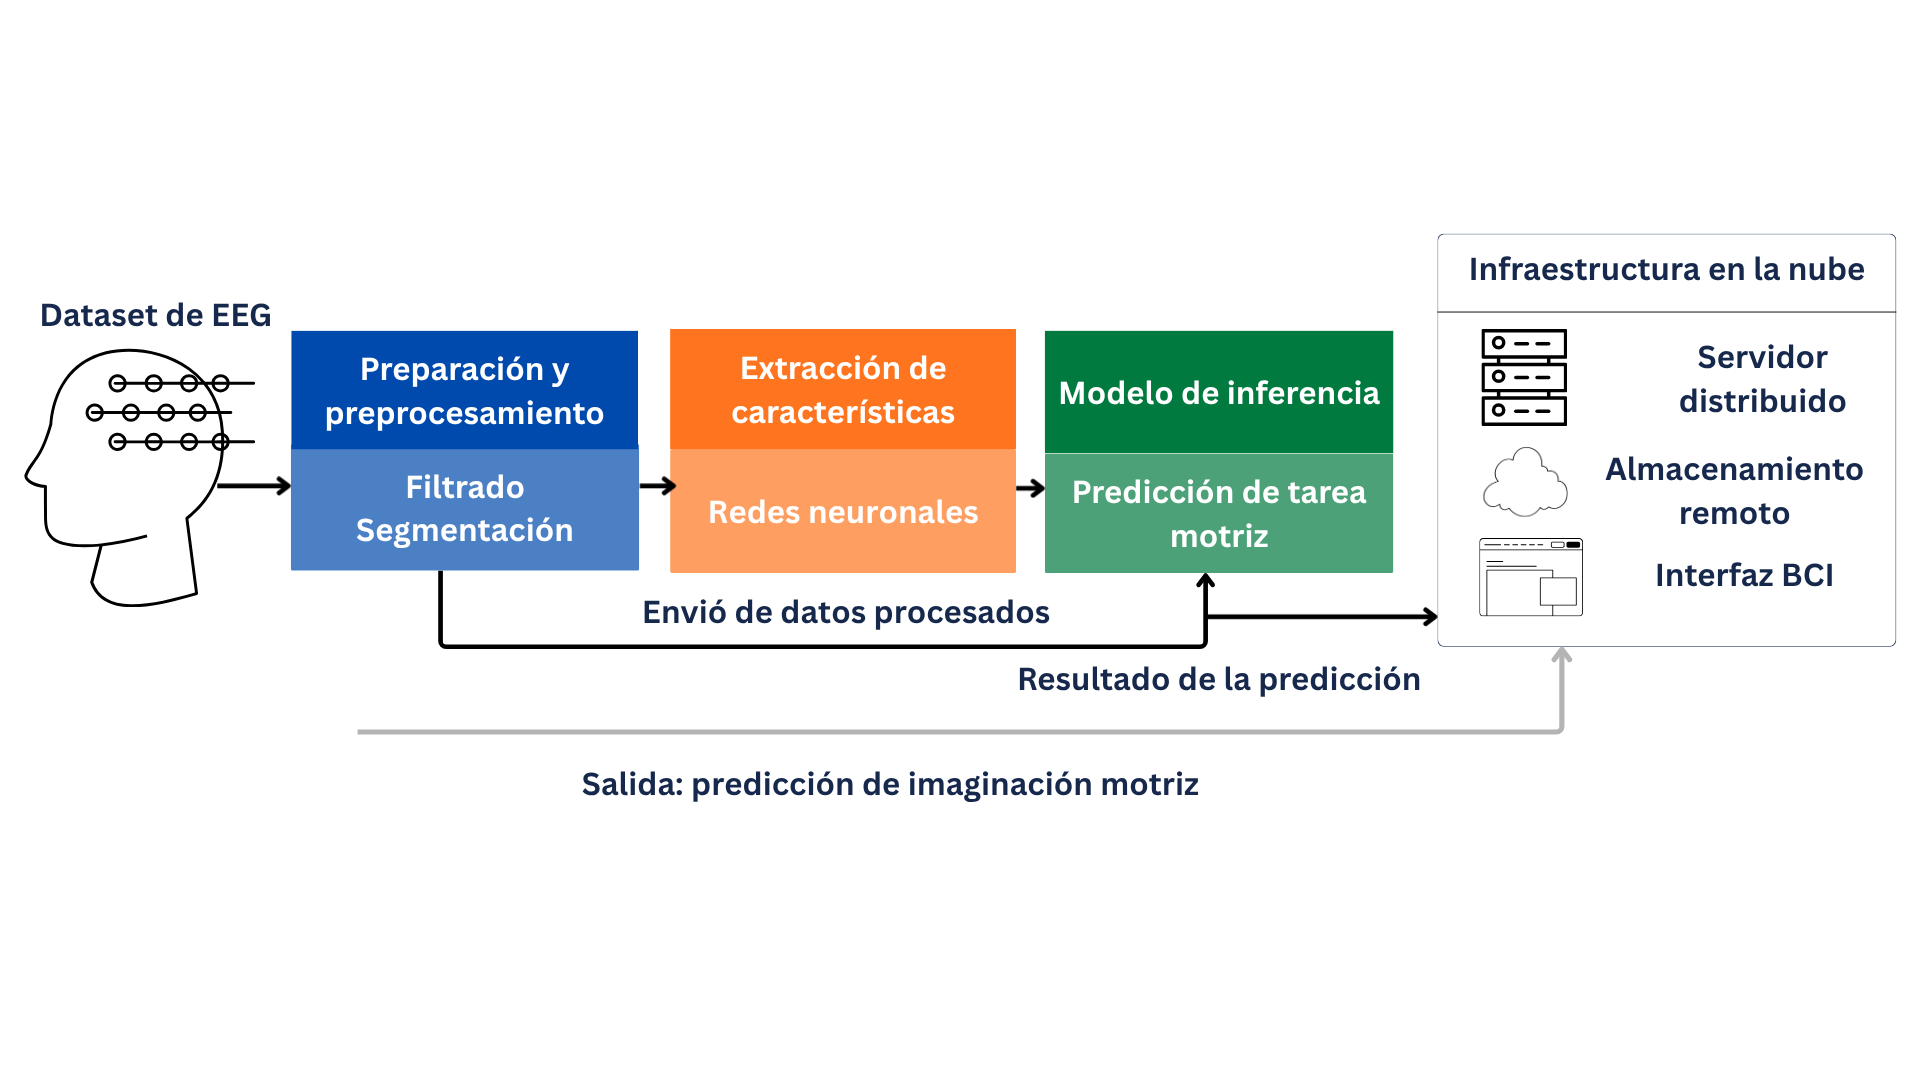
\includegraphics[width=\linewidth]{./Figures/arquitectura-interfaz-cerebro-v2.png}
    % \includegraphics[width=0.8\textwidth]{image_name.pdf} 
    \caption{Diagrama de la arquitectura general del sistema.}
	\label{fig:cloud-arquitecturas}
\end{figure}


Finalmente, el sistema se desplegó bajo un paradigma cloud, que permitió desacoplar el procesamiento intensivo del entorno local. Esta arquitectura facilitó la implementación de una interfaz cerebro-computador cloud, en la que las señales fueron procesadas de manera remota para la generación de resultados.

La arquitectura descrita estableció un flujo completo desde la preparación de los datos hasta la obtención de predicciones, garantizando modularidad, escalabilidad y capacidad de integración con aplicaciones externas.

%----------------------------------------------------------------------------------------
%	SECTION 2
%----------------------------------------------------------------------------------------


\section{Preparación y preprocesamiento de los datos}

En esta sección se describen los métodos aplicados a las señales EEG antes del entrenamiento de los modelos, incluyendo las etapas de preparación, preprocesamiento, filtrado, segmentación, transformación y estandarización de los datos.

\subsection{Preparación de los datos}

En la etapa de preparación, se realizó la carga de los registros EEG considerando su organización estructurada por sujetos, sesiones y ensayos, conforme a la definición del conjunto de datos Dreyer2023A descrito en \cite{dreyer2023large}. Este conjunto incluye múltiples participantes sometidos a experimentos de imaginación motriz de mano izquierda y derecha, con un número significativo de ensayos por sesión, lo que permitió disponer de un volumen amplio de datos para el entrenamiento de los modelos . Por medio de la interfaz de MOABB (del inglés, \textit{Mother Of All BCI Benchmarks}), se accedió a los datos en un formato estandarizado basado en eventos, lo que facilitó la manipulación de las señales y su integración en el flujo de procesamiento.

Después, se identificaron los eventos asociados a cada tarea de imaginación motriz, que correspondían a etiquetas discretas como mano izquierda y mano derecha dentro del paradigma de clasificación binaria . Estos eventos permitieron segmentar las señales continuas en ensayos individuales alineados temporalmente con los estímulos experimentales. Cada ensayo representó una instancia etiquetada del conjunto de datos, lo que permitió estructurar la información en un esquema supervisado ideal para el entrenamiento de los modelos.

Por otra parte, se consideró la consistencia en la organización de los canales EEG y la sincronización temporal de las señales, garantizando que cada muestra mantuviera la correspondencia entre dimensiones espaciales y temporales. Este proceso permitió transformar los datos originales en una representación homogénea, facilitando su posterior procesamiento y asegurando la compatibilidad en terminos de entradas estructuradas y uniformes con los modelos.

\subsection{Preprocesamiento de los datos}

En la fase de preprocesamiento, se aplicó un filtrado de las señales EEG con el objetivo de mejorar la relación señal y ruido para resaltar los componentes relevantes para la tarea de clasificación. Para eso, se empleó un filtro pasa banda en el rango de 8 a 30 Hz, se considera que este intervalo abarca las bandas $\mu$ (aproximadamente 8–13 Hz) y $\beta$ (13–30 Hz), que están estrechamente relacionadas con la actividad cortical asociada a la imaginación motriz \cite{pfurtscheller2001motor, zhang2021eeg}. Estas bandas presentan patrones característicos de desincronización y sincronización relacionados con la ejecución o imaginación de movimientos, lo que las convierte en una fuente relevante de información discriminativa.

El filtrado permitió atenuar componentes de muy baja frecuencia, asociadas a derivas de la señal y artefactos fisiológicos como la actividad electrodermal, así como reducir el ruido de alta frecuencia proveniente de interferencias externas o actividad muscular no deseada. De esta manera, se preservó la información espectral de interés mientras se eliminaban componentes irrelevantes para la tarea.

De igual forma, este proceso contribuyó a estabilizar la señal y a reducir la variabilidad no deseada entre ensayos, que facilitó la posterior etapa de segmentación y el aprendizaje de patrones por parte de los modelos. El filtrado aplicado se mantuvo consistente para todos los sujetos y sesiones, además, se garantizó uniformidad en el tratamiento de los datos y se evitó posibles sesgos introducidos por diferencias en el preprocesamiento. 

\subsection{Segmentación de los datos}

En la fase de segmentación, se realizó la segmentación temporal de las señales EEG en ventanas alineadas con los eventos de estímulo, con el fin de aislar los intervalos de interés asociados a cada tarea de imaginación motriz. A partir de los registros continuos, se extrajeron segmentos (epochs) definidos en un intervalo temporal específico posterior a la aparición del estímulo, asegurando que cada ventana contuviera la respuesta cerebral relevante para la tarea. Este procedimiento permitió sincronizar las señales en relación con el inicio del evento, garantizando coherencia temporal entre las muestras.

Cada segmento fue definido con una duración fija, que permitió obtener representaciones homogéneas en términos de longitud temporal. Esta procedimiento resultó muy útil para su posterior utilización en los modelos, que requieren entradas con dimensiones consistentes. De igual forma, se evitó la inclusión de intervalos previos al estímulo que no aportaran información discriminativa, enfocando el análisis en las regiones temporales donde se manifiestan patrones asociados a la imaginación motriz.

La segmentación generó múltiples muestras independientes a partir de cada registro continuo, se incrementó el número de ejemplos disponibles para el entrenamiento. Este incremento en la cantidad de datos permitió mejorar la capacidad de generalización de los modelos, al exponerlos a una mayor variabilidad intra e intersujeto.

Adicionalmente, se mantuvo la correspondencia entre cada segmento y su respectiva etiqueta de clase, preservando la integridad del conjunto de datos supervisado. Este proceso permitió transformar las señales EEG continuas en un conjunto estructurado de muestras etiquetadas, adecuado para su utilización en tareas de clasificación.

En la tabla \ref{tab:preprocesamiento-data}, se presentan los parámetros utilizados durante las etapas de preparación y preprocesamiento de las señales EEG.

\begin{table}[h]
\centering
\caption[Parámetros Dataset]{Parámetros de preparación y preprocesamiento de \mbox{señales} EEG}
\label{tab:preprocesamiento-data}
\begin{tabular}{|l|l|l|}
\hline
\textbf{Etapa} & \textbf{Parámetro} & \textbf{Valor} \\ \hline

\multirow{10}{*}{Preparación} 
& Dataset & Dreyer2023  \\ \cline{2-3}
& Acceso a datos & MOABB  \\ \cline{2-3}
& Número de sujetos & 60 \\ \cline{2-3}
& Tipo de tarea & Imaginación motriz \\ \cline{2-3}
& Clases & Mano izquierda / Mano derecha \\ \cline{2-3}
& Número de canales EEG & 27 \\ \cline{2-3}
& Sistema de electrodos & 10-20 \\ \cline{2-3}
& Frecuencia de muestreo & 512 Hz \\ \cline{2-3}
& Número de runs por sesión & 6 \\ \cline{2-3}
& Ensayos por run & 40 \\ \hline

\multirow{4}{*}{Preprocesamiento}
& Tipo de señal & Señales crudas \\ \cline{2-3}
& Filtro aplicado & Pasa banda \\ \cline{2-3}
& Rango de filtrado & 8--30 Hz \\ \cline{2-3}
& Bandas analizadas & $\mu$ (8--13 Hz), $\beta$ (13--30 Hz) \\ \hline

\multirow{3}{*}{Segmentación}
& Tipo de ventana & Epochs alineados a estímulo \\ \cline{2-3}
& Intervalo temporal & Posterior al estímulo \\ \cline{2-3}
& Duración de ventana & Fija \\ \hline

Normalización & Tipo & Estandarización por muestra \\ \hline

Estructuración & Formato de entrada & (canales $\times$ tiempo) \\ \hline

\end{tabular}
\end{table}